\subsection{kort introduktion til prototype}
(hvorfor har vi valt lige disse billeder, eventuel noget med, der er mange hovder så der er nok også en vis cance for at der finder en hovde. lala
)
Ud fra de karakteriseringer som er beskravet i rapporten. få vi
produceret noget data, som omhandler tilblivelsen af region i et snit og
hvor mange der regioner der befinder sig. I dette afsnit vil vi vise
hvad vores prototype er kommet frem til. Ved at se på et vis række billeder
som illustrer hvad der sker i programmet, i grove trak. Der efter vil vi
konkludere, metode god og dårlige eneskaber, og om der kan gøres noget for at
forbedre på fremgangsmåden.


\subsection{Noget smart, kan bare ikke komme på det}
Nå et billedet bearbejdes, i vores program, er der 2 naturlige steder
hvor det vil være fornuftige at se om hvad der sker. Det første er efter vi har
iteraret hen over et af de 4 cut og fundet alle de regioner som ligger
på eller lige omkring snittet.

\begin{figure}[h!!]
	\begin{center}
		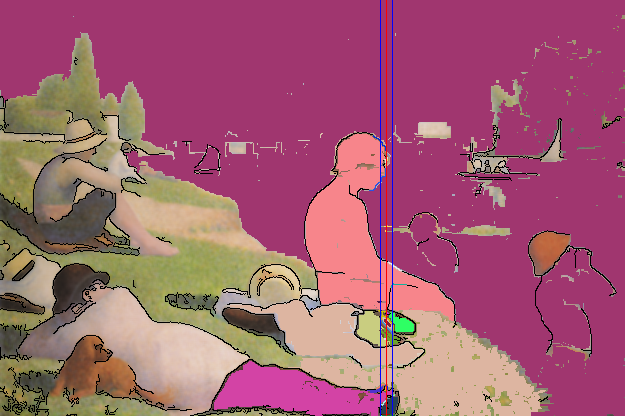
\includegraphics[scale=0.42,angle=0]{afsnit/afprovning/billeder/floodfillbilledet.png}
	\end{center}
	\caption[]{Billedet hvor vores algoritme har fundet x antal regioner}
	\label{ff}
\end{figure}

I billedet \ref{ff} er vær region, indtegnet med vær sin farve, og snittet
som er beregnet ud fra er det horisontale gyldne snit som ligger mest
til højre. Som man kan se finder algoritmen en masse regioner, hvor
nogle af dem er ret spændene at se på, som f.eks. drengen som er farvet
helt lyserød. Der bliver også fundet en masse regioner som ikke er
særlige spændene, f.eks. helle baggrunden som er malet mørkelilla i
billedet. Som man kan af billedet, er der ikke særlige mange regioner, i
selve snittet som bliver tværet ud og kommer til at falde i et med et af
de andre regioner i billedet, det er et godt tegn, da sammensmeltningen af
regioner vil give en forkert fortolkning af billedet.

Det andet naturlige sted at se på, er nå vi tager alle de regioner som
blev fundet og sortere, dem fra, som ikke passer overens med vores
definition, af om regionen ligger i snittet. De regionerne som er taget
med, bliver inremmet i en bos og kan ses på billedet \ref{ff}. 

\begin{figure}[h!!]
	\begin{center}
		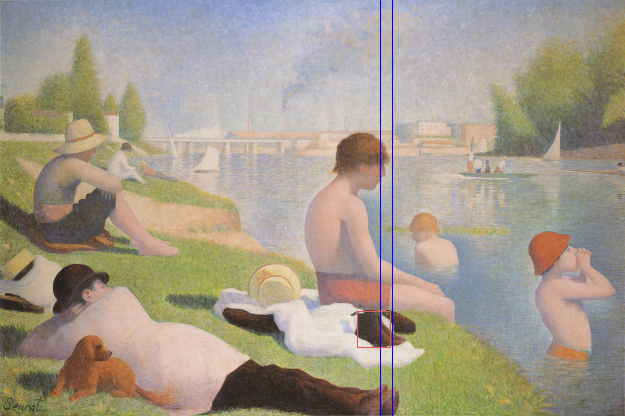
\includegraphics[scale=0.42,angle=0]{afsnit/afprovning/billeder/boindingboxbilledet.png}
	\end{center}
	\caption[]{Billedet de regioner som vi har tilbage, er i en box}
	\label{blob}
\end{figure}

Som man kan se er der kun 1 region tilbage, som omkredser en sko i
billedet. Men tilgængel er alle de store regioner så som baggrunden og
græsset ikke blevet taget med. Det kan både siges at være godt og skidt.
det gode er at vi nu har en god ide om, hvad der bliver fundet. hvis vi
samme liner vores beskrivelse af vores fremgangsmåde, og hvordan
billedet ser ud. Stemmer det over ens, så vores algoritme virker skulle virke. Det
dårlige er, at vi fjerner ret meget. F.eks. kunne drengen være en
region som man gerne vil have med.

For at give lidt parspiktic, vil jeg også visser vi et par andet billedet, hvor
vores metode opføre sig en kende anderledes.
	
\begin{figure}[h!!]
	\begin{center}
		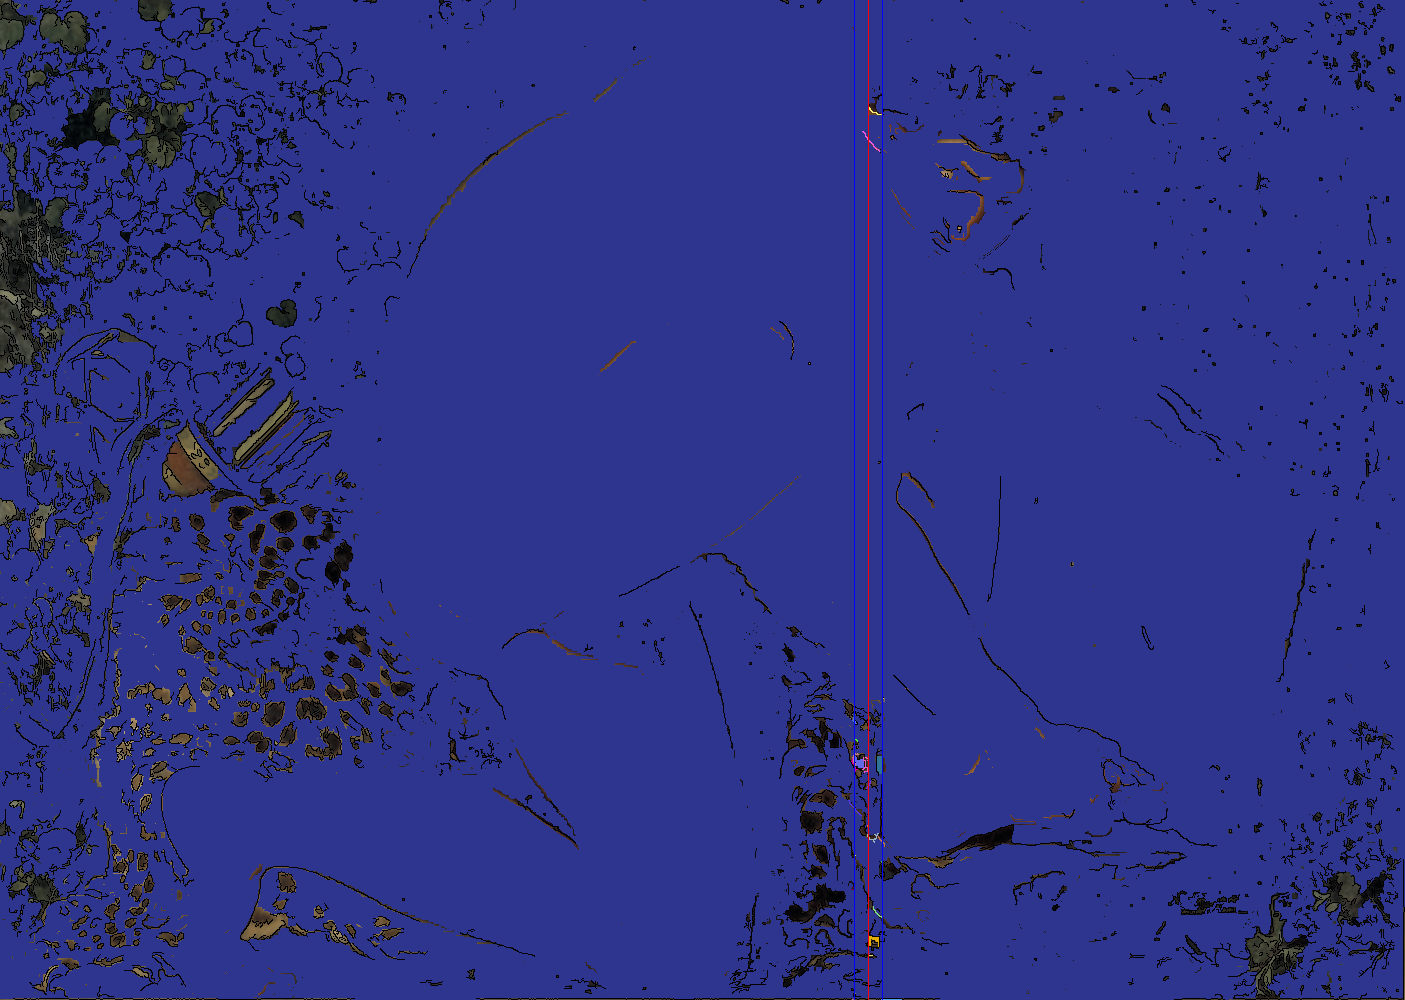
\includegraphics[scale=0.20,angle=0]{afsnit/afprovning/billeder/nicofloodfillbilledet.png}
	\end{center}
	\caption[]{Som man kan se på billedet, er der kun en stor region.
	           Grunden til dette er at billedet er af en anden kunstner
	           og er blevet lidt gråligt, efter alle de år på muserum,
	           så farverne ligger ikke særlige lang for hinanden. Dette
	           få vores metode til at fejle en kende.}
	\label{nicofill}
\end{figure}

\begin{figure}[h!!]
	\begin{center}
		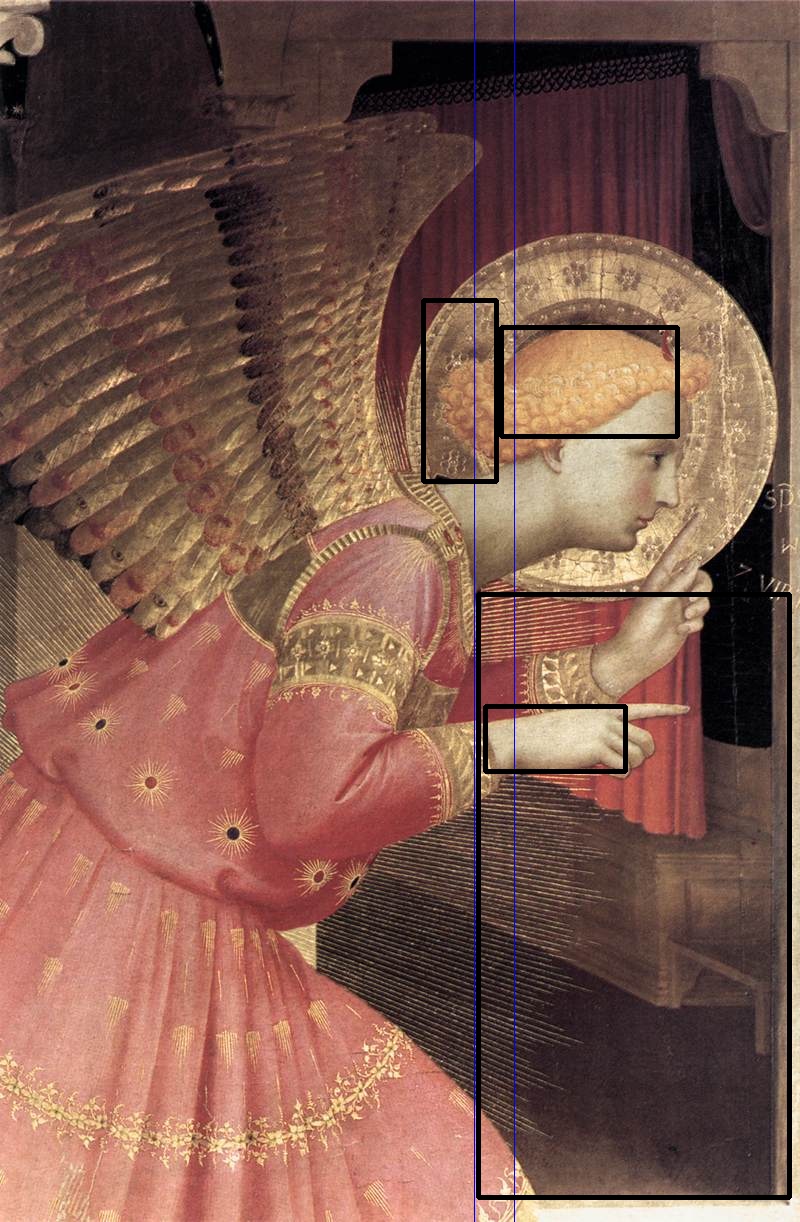
\includegraphics[scale=0.30,angle=0]{afsnit/afprovning/billeder/BB1annunc2.png}
	\end{center}
	\caption[]{Billedet af en engel, hvor noget af glorien og hinden
	           hånd er fundet. som det kan ses ligger hånden efter vores
	           defination i det gyldne snit, og er en ret interasat
	           ting, da hånden viser hvad engelen hendtyr, selve glorien
	           er også i interasant, men ligger ikke i snittet, så det
	           er lidt uheldig at vi finder en fraktion af dem.}
	\label{BB1annunc2}
\end{figure}

\begin{figure}[h!!]
	\begin{center}
		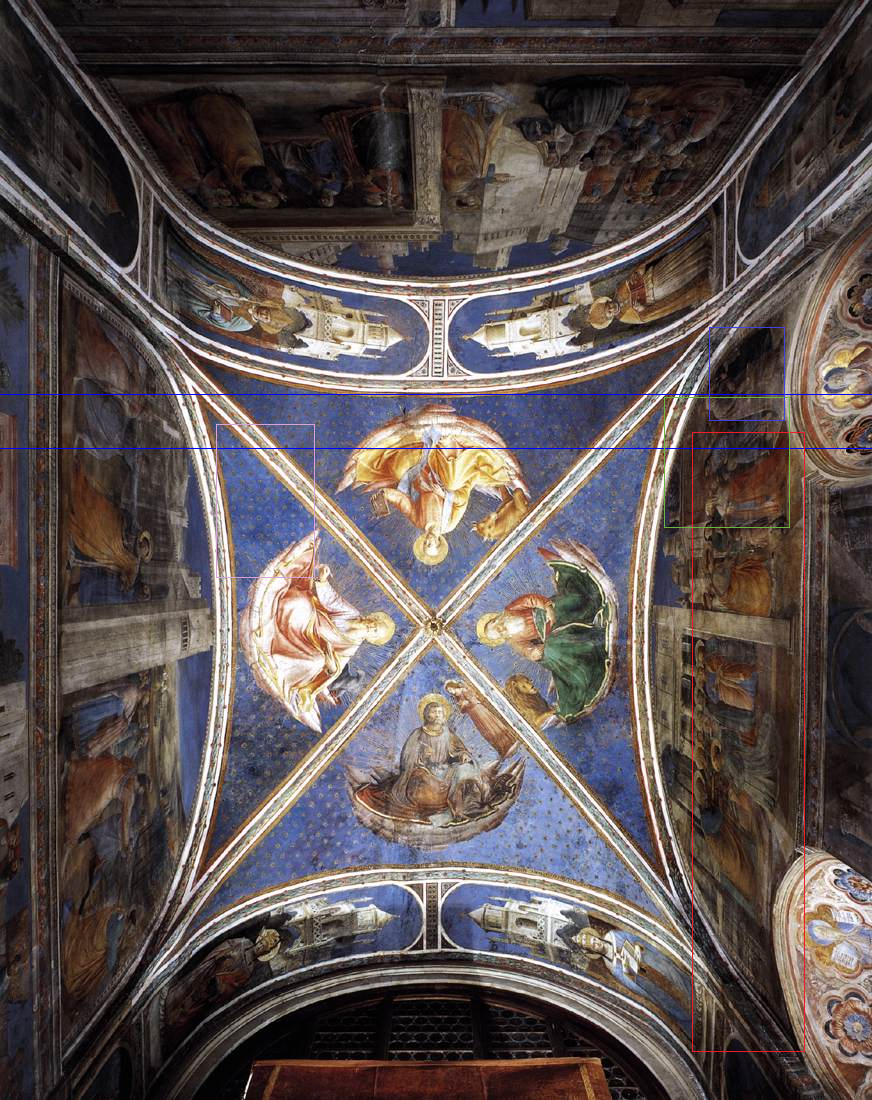
\includegraphics[scale=0.30,angle=0]{afsnit/afprovning/billeder/BB3vault.png}
	\end{center}
	\caption[]{I dette billedet er der mallet et loft, og vores metode
	          finde kun ting som ikke er serlige fede at have med}
	\label{BB3vault}
\end{figure}

\begin{figure}[h!!]
	\begin{center}
		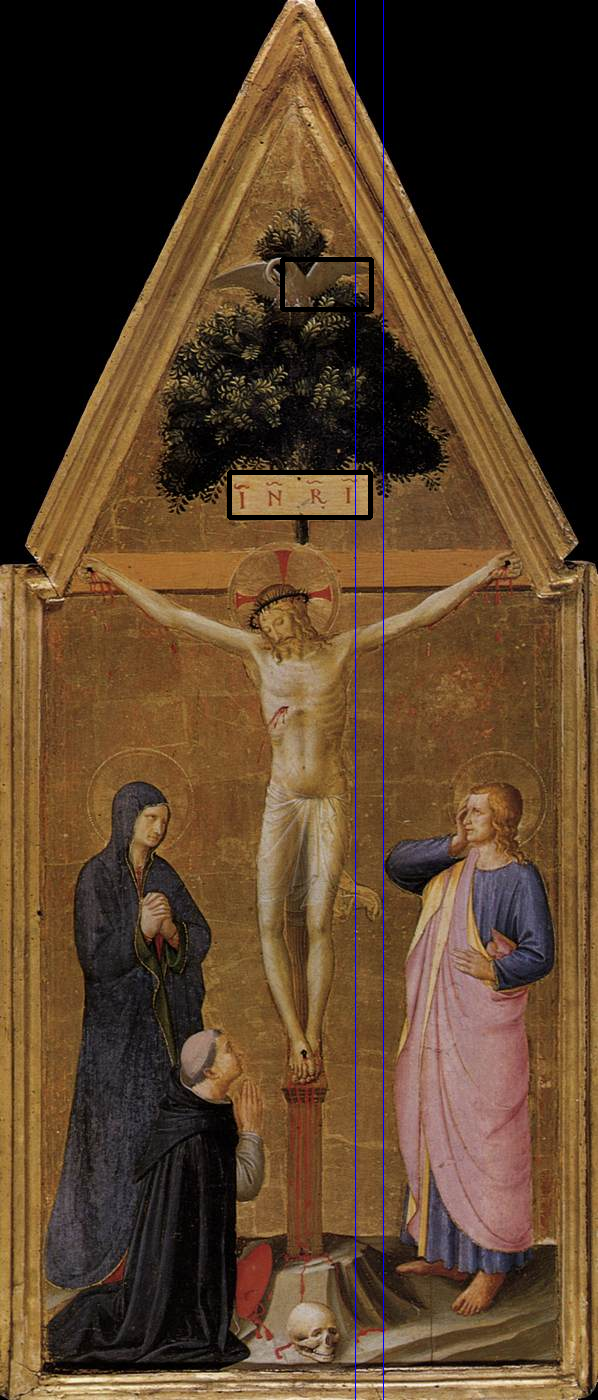
\includegraphics[scale=0.30,angle=0]{afsnit/afprovning/billeder/BB09crucif.png}
	\end{center}
	\caption[]{Metoden finder i dette billedet svanen, som er en meget
	           framtradene ting i billedet, metoden finder også skildet,
	           selve om det er svært at se, dette er et ret god eksempel
	           på at vore metode faktisk finder nogle lunde pracice
	           ragioner, dog kan man se at metoden ikke har det så god
	           nå vi arbejder på firkandet billeder}
	\label{BB09crucif}
\end{figure}

\begin{figure}[h!!]
	\begin{center}
		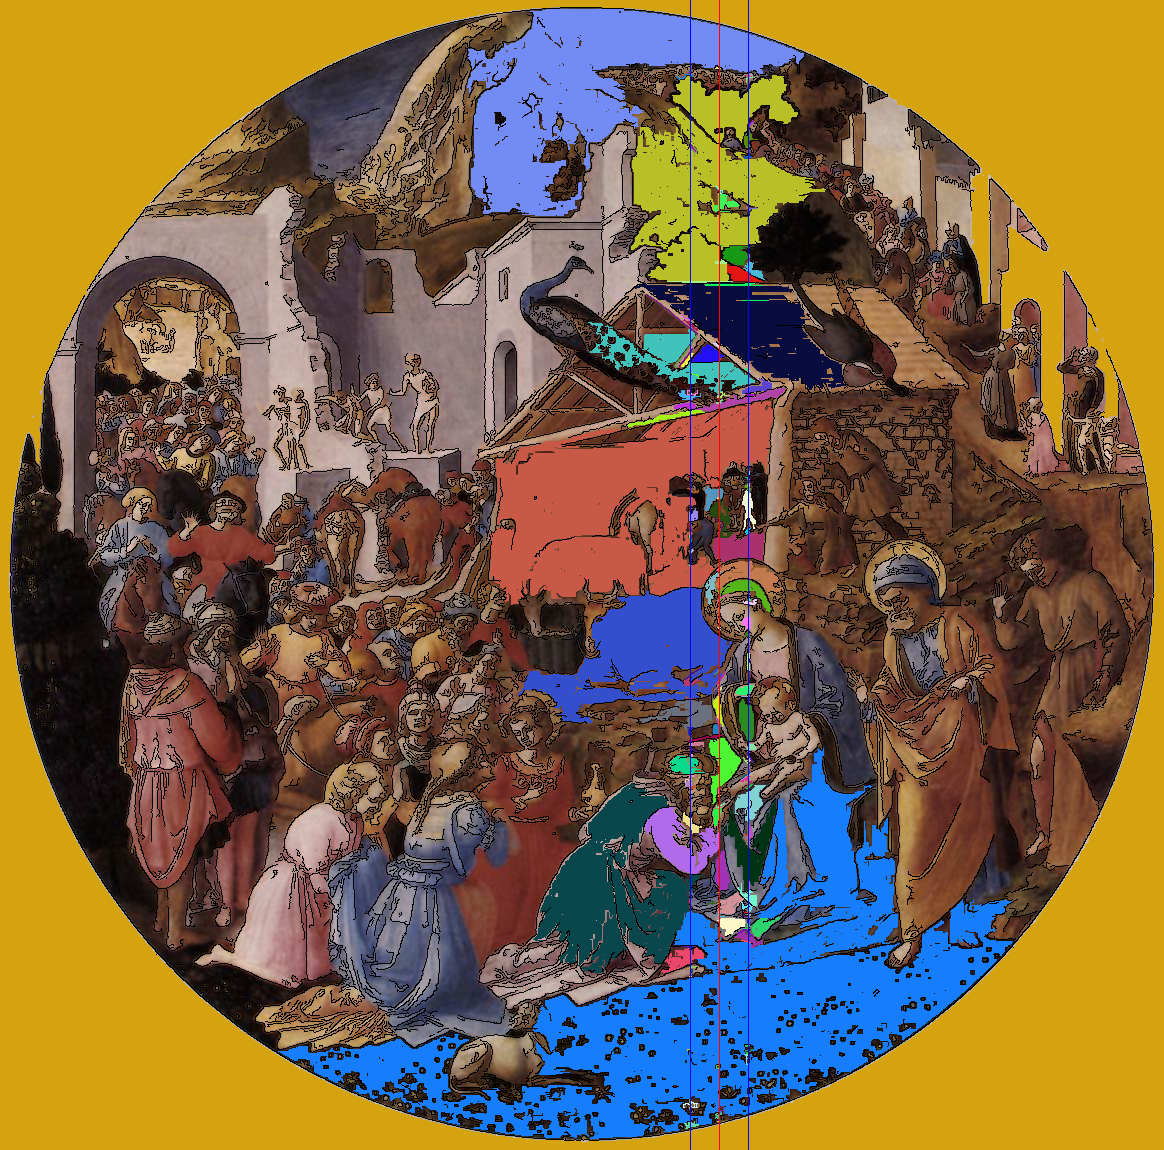
\includegraphics[scale=0.3,angle=0]{afsnit/afprovning/billeder/FFadorat.png}
	\end{center}
	\caption[]{Dette floodfillet billedet, vise at selv om vi har en
	           metode som virker ok, så har vi stadig problemer nå
	           billedet er rundt og ikke gå helt ud til kanten af
	           rammen, få det ser faktisk ud som om kvinden og manden
	           ligger i snittet. Men dette kan ændre sig meget, da det
	           snit som er tegnet ind, er udregnet ud fra kanten af
	           rammen, og ikke billedet kant.}
	\label{FFadorat}
\end{figure}

\begin{figure}[h!!]
	\begin{center}
		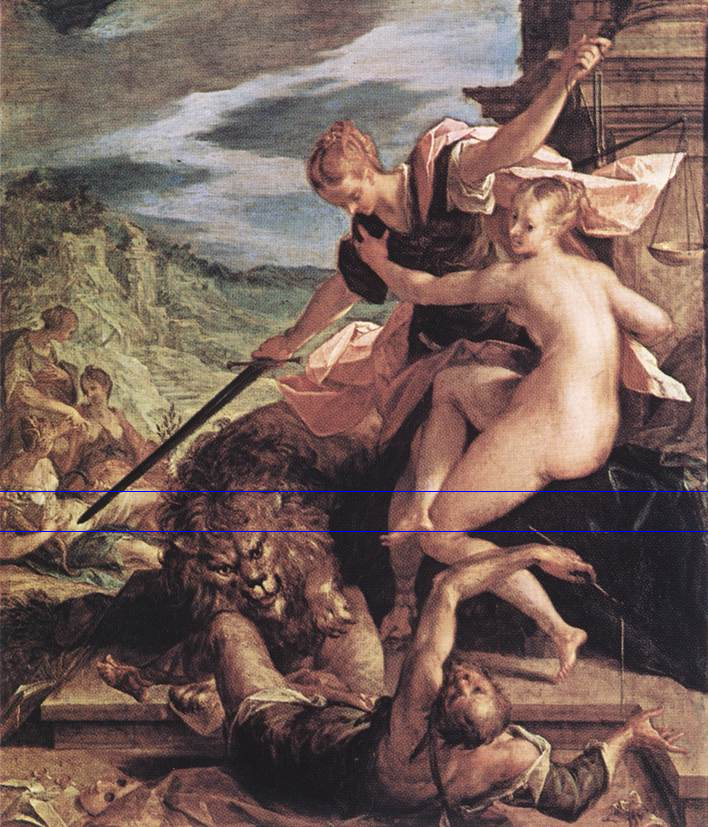
\includegraphics[scale=0.50,angle=0]{afsnit/afprovning/billeder/BBallegory.png}
	\end{center}
	\caption[]{Dette er et fantastisk eksempel på at der ikke ligger
	           noget som helst i dette snit, og der er heller ikke
	           findet nogle ragioner i snittet.}
	\label{BBallegory}
\end{figure}

\begin{figure}[h!!]
	\begin{center}
		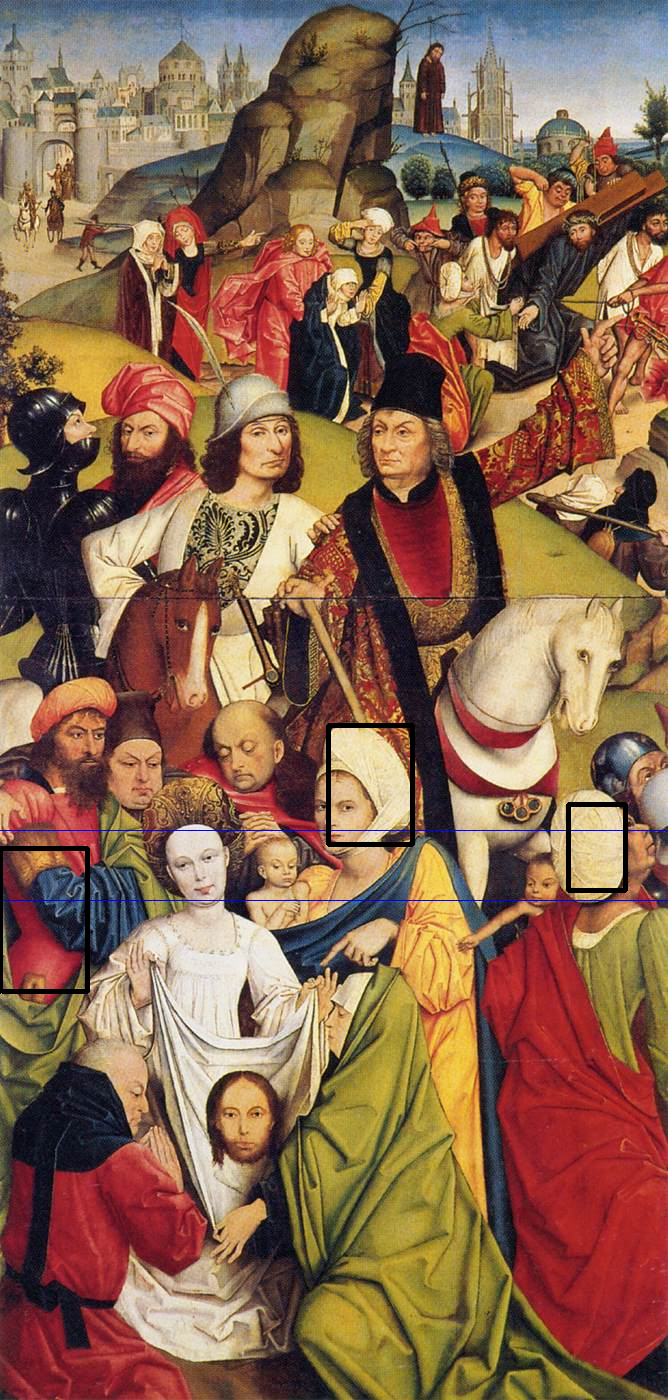
\includegraphics[scale=0.35,angle=0]{afsnit/afprovning/billeder/BBCarruingcut2.png}
	\end{center}
	\caption[]{I dette billedet finder vi 4 ragioner som ligger i det
	           gyldne snit, 3 hovder og et barne omris. Dette passer god}
	\label{BBCarruingcut2}
\end{figure}

\begin{figure}[h!!]
	\begin{center}
		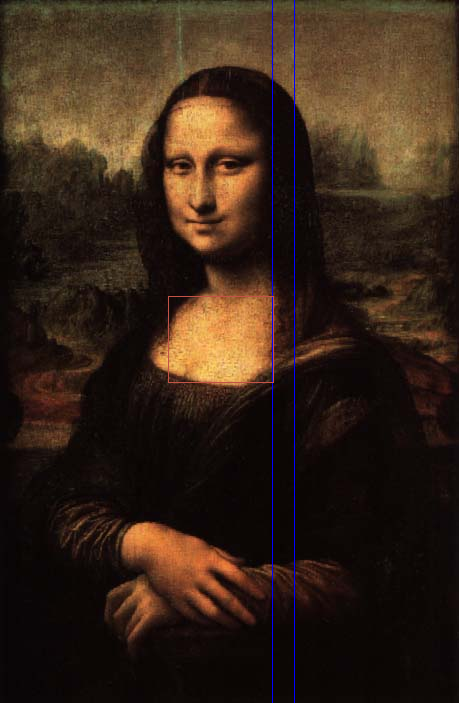
\includegraphics[scale=0.50,angle=0]{afsnit/afprovning/billeder/BBMonalisacut0.png}
	\end{center}
	\caption[]{Mona lisa i et af de 2 snit, hvor ikke hindes andsikt bliver fundet, men hindes øverstebryst, som også er ret framhøvet i  billedet}
	\label{BBMonalisacut0}
\end{figure}

\begin{figure}[h!!]
	\begin{center}
		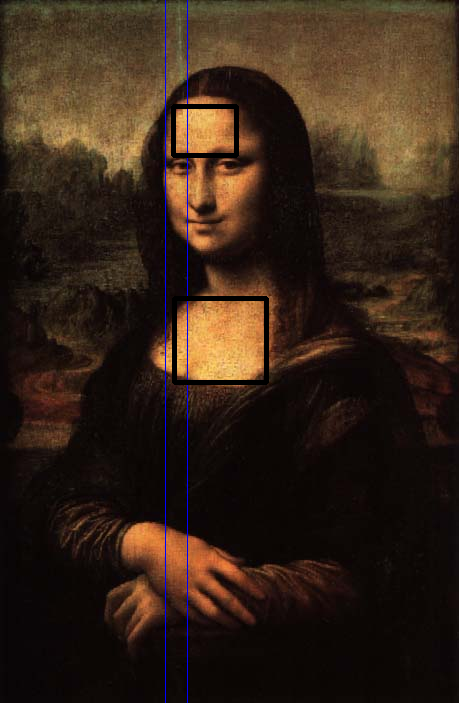
\includegraphics[scale=0.50,angle=0]{afsnit/afprovning/billeder/BBMonalisacut1.png}
	\end{center}
	\caption[]{Monalisa med et andet cut, hvor det sammen er blevet fundet, dette tyder på at vi har en motode som er konsistens med hvad den finder}
	\label{BBMonalisacut1}
\end{figure}


\subsection{hvad kan vi gøre bedre}
I det første billedet \ref{ff}, mener vi at den ting som virkelige kan
forbedre måde vores metode arbejder på. Er ved at ændre på den
definition som sortere regioner fra. Så en region kan krydse begge
marginer. Den anden ting man kunne se på, omhandler det andet billedet
\ref{nicofill}, hvor vi få for meget med, dette kunne løses ved at se på
individuelde billeder og regne ud hvor meget algoritmerne må tage med.
Begge disse to forslag vil blive diskuteret yderligt i den udvidet
løsning af problemet, hvor vi vil gå ind på hvad vi gør for at kommer
over nogle at de problemer som vi har.
